\documentclass[conference]{IEEEtran}
\usepackage[utf8]{inputenc}

% Graphics
\usepackage[pdftex]{graphicx}
\DeclareGraphicsExtensions{.pdf,.jpeg,.jpg,.png,.svg}
\usepackage{caption}
\usepackage{subcaption}

\usepackage{rotating}
\usepackage{tabularx}

\ifCLASSOPTIONcompsoc
\usepackage[caption=false,font=normalsize,labelfont=sf,textfont=sf]{subfig}
\else
\usepackage[caption=false,font=footnotesize]{subfig}
\fi

% To use inline and other fancy list-like environments (e.g., inparaenum)
\usepackage{paralist}

% For smart references
\usepackage{cleveref}
\crefname{algocf}{Algorithm}{Algorithms}
\crefname{figure}{figure}{figures}
\crefname{missingfigure}{fig.}{figs.}

\usepackage[nonumberlist,acronym]{glossaries}

%% Add-ons
%% Declare and Target-Branched Declare
\def\btarget {Target-Branched}
\def\btargetdeclare {{\btarget} Declare}
\def\btargetdeclarecon {{\btargetdeclare} constraint}
\def\declare {Declare}
\def\reldeclare {Relation Declare}
\def\btargetdeclarecontem {{\btargetdeclare} constraint template}
\def\branchfactor {branching factor}
\def\ltlf {LTL$_f$}

% MINERful stuff
\def\minerfulKB {\ensuremath{\mathcal{KB}}}
\def\parakappa {\ensuremath{k^{||}}}
\def\paraqu {\ensuremath{q^{||}}}
\def\kbSum {\ensuremath{\oplus}}

%
\def\GenericTmp {\ensuremath{\mathcal{C}}}
\def\GenericPrimeTmp {\ensuremath{\mathcal{C}'}}
\def\GenericSecondTmp {\ensuremath{\mathcal{C}''}}
%
\newcommand{\GenericRelCns}[2] {\ensuremath{\mathcal{C}(#1,#2)}}
\newcommand{\GenericPrimeRelCns}[2] {\ensuremath{\mathcal{C}'(#1,#2)}}
\newcommand{\GenericSecondRelCns}[2] {\ensuremath{\mathcal{C}''(#1,#2)}}

\def\PartTxt {Participation}
\def\UniqTxt {AtMostOne}
\def\InitTxt {Init}
\def\EndTxt {End}
\def\ResExTxt {RespondedExistence}
\def\RespTxt {Response}
\def\AltRespTxt {AlternateResponse}
\def\ChaRespTxt {ChainResponse}
\def\PrecTxt {Precedence}
\def\AltPrecTxt {AlternatePrecedence}
\def\ChaPrecTxt {ChainPrecedence}
\def\CoExiTxt {CoExistence}
\def\SuccTxt {Succession}
\def\AltSuccTxt {AlternateSuccession}
\def\ChaSuccTxt {ChainSuccession}
\def\NotCoExiTxt {NotCoExistence}
\def\NotSuccTxt {NotSuccession}
\def\NotChaSuccTxt {NotChainSuccession}

\def\PartTmp {$\mathit{\PartTxt}$}
\def\UniqTmp {$\mathit{\UniqTxt}$}
\def\InitTmp {$\mathit{\InitTxt}$}
\def\EndTmp {$\mathit{\EndTxt}$}
\def\ResExTmp {$\mathit{\ResExTxt}$}
\def\RespTmp {$\mathit{\RespTxt}$}
\def\AltRespTmp {$\mathit{\AltRespTxt}$}
\def\ChaRespTmp {$\mathit{\ChaRespTxt}$}
\def\PrecTmp {$\mathit{\PrecTxt}$}
\def\AltPrecTmp {$\mathit{\AltPrecTxt}$}
\def\ChaPrecTmp {$\mathit{\ChaPrecTxt}$}
\def\CoExiTmp {$\mathit{\CoExiTxt}$}
\def\SuccTmp {$\mathit{\SuccTxt}$}
\def\AltSuccTmp {$\mathit{\AltSuccTxt}$}
\def\ChaSuccTmp {$\mathit{\ChaSuccTxt}$}
\def\NotCoExiTmp {$\mathit{\NotCoExiTxt}$}
\def\NotSuccTmp {$\mathit{\NotSuccTxt}$}
\def\NotChaSuccTmp {$\mathit{\NotChaSuccTxt}$}

\newcommand{\Part}[1] {\ensuremath{\mathit{\PartTxt}(#1)}}
\newcommand{\Uniq}[1] {\ensuremath{\mathit{\UniqTxt}(#1)}}
\newcommand{\Init}[1] {\ensuremath{\mathit{\InitTxt}(#1)}}
\newcommand{\End}[1] {\ensuremath{\mathit{\EndTxt}(#1)}}
\newcommand{\ResEx}[2] {\ensuremath{\mathit{\ResExTxt}(#1,#2)}}
\newcommand{\Resp}[2] {\ensuremath{\mathit{\RespTxt}(#1,#2)}}
\newcommand{\AltResp}[2] {\ensuremath{\mathit{\AltRespTxt}(#1,#2)}}
\newcommand{\ChaResp}[2] {\ensuremath{\mathit{\ChaRespTxt}(#1,#2)}}
\newcommand{\Prec}[2] {\ensuremath{{\mathit{\PrecTxt}}(#1,#2)}}
\newcommand{\AltPrec}[2] {\ensuremath{\mathit{\AltPrecTxt}(#1,#2)}}
\newcommand{\ChaPrec}[2] {\ensuremath{\mathit{\ChaPrecTxt}(#1,#2)}}
\newcommand{\CoExi}[2] {\ensuremath{\mathit{\CoExiTxt}(#1,#2)}}
\newcommand{\Succ}[2] {\ensuremath{\mathit{\SuccTxt}(#1,#2)}}
\newcommand{\AltSucc}[2] {\ensuremath{\mathit{\AltSuccTxt}(#1,#2)}}
\newcommand{\ChaSucc}[2] {\ensuremath{\mathit{\ChaSuccTxt}(#1,#2)}}
\newcommand{\NotCoExi}[2] {\ensuremath{\mathit{\NotCoExiTxt}(#1,#2)}}
\newcommand{\NotSucc}[2] {\ensuremath{\mathit{\NotSuccTxt}(#1,#2)}}
\newcommand{\NotChaSucc}[2] {\ensuremath{\mathit{\NotChaSuccTxt}(#1,#2)}}

\newcommand{\ResExNoMath}[2] { \ResExTmp$($\textit{#1},\textit{#2}$)$ }
\newcommand{\RespNoMath}[2] { \RespTmp$($\textit{#1},\textit{#2}$)$ }
\newcommand{\AltRespNoMath}[2] { \AltRespTmp(\textit{#1},\textit{#2}) }
\newcommand{\ChaRespNoMath}[2] { \ChaRespTmp(\textit{#1},\textit{#2}) }
\newcommand{\PrecNoMath}[2] { \PrecTmp(\textit{#1},\textit{#2}) }
\newcommand{\AltPrecNoMath}[2] { \AltPrecTmp(\textit{#1},\textit{#2}) }
\newcommand{\ChaPrecNoMath}[2] { \ChaPrecTmp(\textit{#1},\textit{#2}) }

\newcommand{\BranchedTargetNoMath}[1] {$\lbrace$#1$\rbrace$}
\newcommand{\BranchedTarget}[1] { \ensuremath{\lbrace#1\rbrace} }

\def\DistFunctor { \ensuremath{ \delta } }
\def\OccuFunctor { \ensuremath{ \gamma } }

\newcommand{\DistFunc}[3] { \ensuremath{\DistFunctor_{#1,#2}(#3)} }
\newcommand{\OccuFunc}[2] { \ensuremath{\OccuFunctor_{#1}(#2)} }

\def\NoAfterFunctor { \overset{\nrightarrow}{\delta_0} }
\def\NoBeforeFunctor { \overset{\nleftarrow}{\delta_0} }
\def\NoEverFunctor { \overset{\nleftrightarrow}{\delta_0} }
\def\OneAfterFunctor { \overset{\rightarrow}{\delta_1} }
\def\OneBeforeFunctor { \overset{\leftarrow}{\delta_1} }
\def\RepeatBetweenNextFunctor { \overset{\looparrowright}{\beta} }
\def\RepeatBetweenPrevFunctor { \overset{\looparrowleft}{\beta} }

% \newcommand{\NoAfterFunc}[2] { \ensuremath{ \NoAfterFunctor \left( #1, \widehat{#2} \right) } }
\newcommand{\NoAfterFunc}[2] { \ensuremath{ \NoAfterFunctor \left( #1, #2 \right) } }
\newcommand{\NoBeforeFunc}[2] { \ensuremath{ \NoBeforeFunctor \left( #1, #2 \right) } }
\newcommand{\NoEverFunc}[2] { \ensuremath{ \NoEverFunctor \left( #1, #2 \right) } }
\newcommand{\OneAfterFunc}[2] { \ensuremath{ \OneAfterFunctor \left( #1, #2 \right) } }
\newcommand{\OneBeforeFunc}[2] { \ensuremath{ \OneBeforeFunctor \left( #1, #2 \right) } }
% \newcommand{\RepeatBetweenNextFunc}[2] { \ensuremath{ \RepeatBetweenNextFunctor \left( #1, \widecheck{#2} \right) } }
\newcommand{\RepeatBetweenNextFunc}[2] { \ensuremath{ \RepeatBetweenNextFunctor \left( #1, #2 \right) } }
\newcommand{\RepeatBetweenPrevFunc}[2] { \ensuremath{ \RepeatBetweenPrevFunctor \left( #1, #2 \right) } }

\newcommand{\RepeatFlagNext}[2] { \ensuremath{ \beta^?_{#1, #2} } }
\newcommand{\RepeatCountNext}[2] { \ensuremath{ \mathtt{N}^{\beta}_{#1, #2} } }
\newcommand{\RepeatTargetNext}[2] { \ensuremath{ \beta^{\odot}_{#1, #2} } }
\newcommand{\NevermoreCount}[2] { \ensuremath{ \mathtt{N}^{\nrightarrow}_{#1, #2} } }
\def\DiffSetNevermoreCountFunctor { \mathtt{{\Delta}N}^{\nrightarrow} }
\newcommand{\DiffSetNevermoreCount}[2] { \ensuremath{ \mathtt{{\Delta}N}^{\nrightarrow}_{#1, #2} } }
\newcommand{\NewDiffSetNevermoreCount}[2] { \ensuremath{ \mathtt{{\Delta}N}^{'\nrightarrow}_{#1, #2} } }
\newcommand{\NeverbeforeCount}[2] { \ensuremath{ \mathtt{N}^{\nleftarrow}_{#1, #2} } }
\def\DiffSetNeverbeforeCountFunctor { \mathtt{{\Delta}N}^{\nleftarrow} }
\newcommand{\DiffSetNeverbeforeCount}[2] { \ensuremath{ \mathtt{{\Delta}N}^{\nleftarrow}_{#1, #2} } }
\newcommand{\NewDiffSetNeverbeforeCount}[2] { \ensuremath{ \mathtt{{\Delta}N}^{'\nleftarrow}_{#1, #2} } }
\newcommand{\NeveratallCount}[2] { \ensuremath{ \mathtt{N}^{\nleftrightarrow}_{#1, #2} } }
\def\DiffSetNeveratallCountFunctor { \mathtt{{\Delta}N}^{\nleftrightarrow} }
\newcommand{\DiffSetNeveratallCount}[2] { \ensuremath{ \mathtt{{\Delta}N}^{\nleftrightarrow}_{#1, #2} } }
\newcommand{\NewDiffSetNeveratallCount}[2] { \ensuremath{ \mathtt{{\Delta}N}^{'\nleftrightarrow}_{#1, #2} } }
\newcommand{\RepeatBetweenNextCount}[2] { \ensuremath{ \mathtt{N}^{\looparrowright}_{#1, #2} } }
\def\DiffSetRepeatBetweenNextCountFunctor { \mathtt{{\Delta}N}^{\looparrowright} }
\newcommand{\DiffSetRepeatBetweenNextCount}[2] { \ensuremath{ \mathtt{{\Delta}N}^{\looparrowright}_{#1, #2} } }
\newcommand{\NewDiffSetRepeatBetweenNextCount}[2] { \ensuremath{ \mathtt{{\Delta}N}^{'\looparrowright}_{#1, #2} } }
\newcommand{\NewNewDiffSetRepeatBetweenNextCount}[2] { \ensuremath{ \mathtt{{\Delta}N}^{''\looparrowright}_{#1, #2} } }
\newcommand{\RepeatBetweenPrevCount}[2] { \ensuremath{ \mathtt{N}^{\looparrowleft}_{#1, #2} } }
\def\DiffSetRepeatBetweenPrevCountFunctor { \mathtt{{\Delta}N}^{\looparrowright} }
\newcommand{\DiffSetRepeatBetweenPrevCount}[2] { \ensuremath{ \mathtt{{\Delta}N}^{\looparrowleft}_{#1, #2} } }
\newcommand{\NewDiffSetRepeatBetweenPrevCount}[2] { \ensuremath{ \mathtt{{\Delta}N}^{'\looparrowleft}_{#1, #2} } }
\newcommand{\NewNewDiffSetRepeatBetweenPrevCount}[2] { \ensuremath{ \mathtt{{\Delta}N}^{''\looparrowleft}_{#1, #2} } }
\newcommand{\OneAfterCount}[2] { \ensuremath{ \mathtt{N}^{1\shortrightarrow}_{#1, #2} } }
\newcommand{\OneBeforeCount}[2] { \ensuremath{ \mathtt{N}^{\shortleftarrow 1}_{#1, #2} } }

\newcommand{\NoAppFunc}[1] { \ensuremath{ \overset{\nsim}{\gamma_0} \left( #1 \right) } }
\newcommand{\CounterFunc}[1] { \ensuremath{ \Gamma \left( #1 \right) } }

\newcommand{\taskize}[1] {\ensuremath{\textsf{#1}}}

\def\taska {\taskize{a}}
\def\taskf {\taskize{f}}
\def\taskc {\taskize{c}}
\def\taskn {\taskize{n}}
\def\taskp {\taskize{p}}
\def\taski {\taskize{i}}
\def\taskr {\taskize{r}}
\def\tasks {\taskize{s}}
\def\taskv {\taskize{v}}

\def\taskb {\taskize{b}}
\def\taskx {\taskize{x}}
\def\tasky {\taskize{y}}
\def\taskz {\taskize{z}}


\def\nicksclass {\ensuremath{\mathcal{NC}} }

\def\superscalar {\ensuremath{\mathcal{\mathit{on}}} \xspace }
\def\nosuperscalar {\ensuremath{\mathcal{\mathit{off}}}\xspace }


\def\SupportFunctor {\mathcal{S}}
\def\ConfidenceFunctor {\mathcal{L}}

\newcommand{\SupportFunc}[1] { \ensuremath{\SupportFunctor\left( #1 \right)} }
\newcommand{\ConfidenceFunc}[1] { \ensuremath{\ConfidenceFunctor\left( #1 \right)} }

\def\BranchingFactor { \ensuremath{ \rho } }

% LTL
\def\LTLnext {\ensuremath{\bigcirc}}
\def\LTLfut {\ensuremath{\Diamond}}
\def\LTLglob {\ensuremath{\Box}}
\def\LTLuntil {\ensuremath{\;\mathcal{U}\,}}
\def\LTLwntil {\ensuremath{\;\mathcal{W}\,}}


\newcommand{\Next}{\raisebox{-0.27ex}{\LARGE$\circ$}}
\newcommand{\Wnext}{\raisebox{-0.27ex}{\LARGE$\bullet$}}
%%\newcommand{\Next}{\raisebox{0.4ex}{\tiny$\bigcirc$}}
\newcommand{\Until}{\mathop{\U}}
\newcommand{\Release}{\mathop{\R}}
\newcommand{\Wuntil}{\mathop{\W}}
\newcommand{\true}{\mathit{true}}
\newcommand{\false}{\mathit{false}}
\newcommand{\temptrue}{\mathit{temp\_true}}
\newcommand{\tempfalse}{\mathit{temp\_false}}
%%\newcommand{\ttrue}{\mathtt{true}}
%%\newcommand{\ffalse}{\mathtt{false}}
\newcommand{\Last}{\mathit{Last}}
\newcommand{\Ended}{\mathit{Ended}}
\newcommand{\length}{\mathit{length}}
\newcommand{\last}{\mathit{last}}
\newcommand{\nnf}{\mathit{nnf}}
\newcommand{\CL}{\mathit{CL}}
\newcommand{\MU}[2]{\mu #1.#2}
\newcommand{\NU}[2]{\nu #1.#2}
\newcommand{\BOX}[1]{ [#1]}
\newcommand{\DIAM}[1]{\langle #1 \rangle}


%%%%%%%%%%%%%%%%%%%%%%acronym.tex%%%%%%%%%%%%%%%%%%%%%%%%%%%%%%%%%%%%%%%%%
% sample list of acronyms
%
% Use this file as a template for your own input.
%
%%%%%%%%%%%%%%%%%%%%%%%% Springer %%%%%%%%%%%%%%%%%%%%%%%%%%

\Extrachap{Glossary}


Use the template \emph{glossary.tex} together with the Springer document class SVMono (monograph-type books) or SVMult (edited books) to style your glossary\index{glossary} in the Springer layout.


\runinhead{glossary term} Write here the description of the glossary term. Write here the description of the glossary term. Write here the description of the glossary term.

\runinhead{glossary term} Write here the description of the glossary term. Write here the description of the glossary term. Write here the description of the glossary term.

\runinhead{glossary term} Write here the description of the glossary term. Write here the description of the glossary term. Write here the description of the glossary term.

\runinhead{glossary term} Write here the description of the glossary term. Write here the description of the glossary term. Write here the description of the glossary term.

\runinhead{glossary term} Write here the description of the glossary term. Write here the description of the glossary term. Write here the description of the glossary term.

% For side notes, missing figures and inline to-do's
\usepackage[textsize=scriptsize]{todonotes}

% For enumerating the line numbers
\usepackage[switch]{lineno}
%Multirow tables
\usepackage{multirow}
%Dashed line in tables
\usepackage{arydshln}
\usepackage{booktabs}

\usepackage[section]{placeins}

\usepackage{url}
\urldef{\wumailaddresses}\path|{firstname.lastname}@wu.ac.at|
%\urldef{\wumailaddresses}\path|{thomas.thonhofer,michael.aschauer,saimir.bala, andreas.rogge-solti, jan.mendling}@wu.ac.at|

\begin{document}

\title{Resource Classification from Version Control System Logs}

\author{\IEEEauthorblockN{
      Kushal Agrawal\IEEEauthorrefmark{3},
      Michael Aschauer\IEEEauthorrefmark{1},
      Thomas Thonhofer\IEEEauthorrefmark{1},
Nico Tomsich\IEEEauthorrefmark{2} 
\\
Saimir Bala\IEEEauthorrefmark{1},
Andreas Rogge-Solti\IEEEauthorrefmark{1}
}
\IEEEauthorblockA{
   \IEEEauthorrefmark{3}\tt kushalagrawal1412@gmail.com,\\
   \IEEEauthorrefmark{2}\tt nico.tomsich@gmail.com,\\  \IEEEauthorrefmark{1}\wumailaddresses}
%\IEEEauthorblockA{\IEEEauthorrefmark{2}\tt nico.tomsich@gmail.com}
%\IEEEauthorblockA{\IEEEauthorrefmark{3}\tt kushalagrawal1412@gmail.com}
\IEEEauthorblockA{Wirtschaftsuniversität Wien\\
   Institute for Information Business, Vienna, Austria\\}
}

% make the title area
\maketitle

% As a general rule, do not put math, special symbols or citations
% in the abstract
\begin{abstract}
	Collaboration in business processes and projects requires a division of responsibilities among the participants. Version control systems allow us to collect profiles of the participants that hint at participants' roles in the collaborative work. The goal of this paper is to automatically classify participants into the roles they fulfill in the collaboration. Two approaches are proposed and compared in this paper. The first approach finds classes of users by applying k-means clustering to users based on attributes calculated for them. The classes identified by the clustering are then used to build a decision tree classification model. The second approach classifies individual commits based on commit messages and file types. The distribution of commit types is used for creating a decision tree classification model. The two approaches are implemented and tested against three real datasets, one from academia and two from industry. Our classification covers 86\% percent of the total commits. The results are evaluated with actual role information that was manually collected from the teams responsible for the analyzed repositories.

%This paper documents a research project with the purpose of classifying users of version control systems based on commit logs. The goal is to create an algorithm which does this classification task automatically. The algorithm is implemented in Python, supported by machine learning and natural language processing tools. Two approaches are developed and used throughout the project. The first approach finds classes of users by applying k-means clustering to users based on attributes calculated for them. The classes identified by the clustering are then used to build a decision tree classification model. The second approach classifies individual commits based on commit message and file types. The commit types are aggregated for each user. The distribution of commit types is used for creating a decision tree classification model. The results are evaluated and improved using actual class information gathered from the teams responsible for the analyzed repositories.This is an exploratory study and the results provide insight into the topic and a basis for further research.\\
\end{abstract}
% keywords
\def\IEEEkeywordsname{Keywords}
\begin{IEEEkeywords}
   Role discovery, Version Control Systems, Software Projects
\end{IEEEkeywords}
% For peer review papers, you can put extra information on the cover
% page as needed:
\ifCLASSOPTIONpeerreview
\begin{center} \bfseries EDICS Category: 3-BBND \end{center}
\fi
%
% For peerreview papers, this IEEEtran command inserts a page break and
% creates the second title. It will be ignored for other modes.
\IEEEpeerreviewmaketitle

%\linenumbers
\section{Introduction}\label{sec:introduction}

%Big data is one of the current business trends, but it is not an overnight phenomenon. Companies have always collected immense quantities of data. With technological improvements it is now possible to extract and analyze this new frontier in an efficient way \cite{minelli2012}. This data is created and collected by industry giants as well as the small enterprises and even individual persons via software systems. 
In the field of software engineering, \gls{vcs} such as Git or \gls{svn} have become an indispensable tool and are used for the majority of collaborative development projects. The repositories of these systems store data about projects and their contributors, beyond the raw source code they committed~\cite{Yu.LiguoRamaswamy.2007}.
From a management perspective, it is interesting to analyze repository data for compliance purposes. From an academic perspective, repositories hold valuable information about the way people work and collaborate.
%\todo[inline]{TODO: add more of "why we need this" to this section and add some citations to works that also claim that this is relevant.}

%The increasing popularity of open source software projects and the emergence of VCS repository hosting services such as GitHub or SourceForge has made this data publicly available. 
%For open source projects, anyone can fetch a log file of their revision histories, containing meta information in the form of author names, commit messages, timestamps and lists of added, modified and deleted files. This easily accessible information is just waiting to be analyzed and contains valuable and useful information.
%There are certainly multiple directions to go in, when applying data mining to VCS logs. 

In this paper the focus lies on mining and analyzing properties of the users. More specifically, it aims at classifying the users which appear in the logs. This idea is based on the assumption that different types of users utilize the system in different ways and that these differences are reflected in their commits and subsequently in the logs. More precisely, we are interested in the following research questions:
%For this task we formulated three research questions:


\begin{enumerate}

%\item Is it possible to do a classification based on VCS logs?
\item Is it possible to classify resources from VCS log data?

%\item What classes can be assigned?
\item To what extent can resources be assigned to classes?

%\item What are the main differences found for these classes?
\item What are the main differences among these classes?

\end{enumerate}


The main objective is to find a way of classifying users automatically, using an algorithm built on common data mining and machine learning methods. The devised algorithm answers these research questions.


This paper is structured as follows: Section 2 provides the basis for this paper, links it to related work and formulates the research questions. Section 3 presents two approaches on how users can be classified in version control systems. In Section 4 the implementation of two algorithmic solutions is described, followed by an analysis of the results. Section 5 concludes the paper.


\section{The Problem of Organizational Perspective Discovery}\label{sec:problemDescription}

The problem we address in this section is the discovery of the roles that members of a software project may actually play in a collaborative setting. Each member is assigned to at least one role in the project. Roles are decided in the project planning phase. This phase also involves the definition of project tasks and the assignment of suitable tasks to the various roles. 

Projects follow clear guidelines. Guidelines may come from internal policies or from rules and regulations of the working domain. For example, software systems in the railway domain must make sure that their development process and resources comply with safety requirements imposed by the European standard EN50128. This is why project managers need to track how they distribute work to different people and whether the project members effectively contribute according to their role and their task. 

\Gls*{scm} systems are a valuable source of information to investigate on the behavior of project members. These systems are used for tracking and controlling changes in the software. If a change produces a wrong or undesired outcome, it is always possible to revert to an older configuration of the system. Artifacts' versions are automatically managed by \glspl*{vcs}. It is always possible to follow the evolution of each artifact, along with information about the resources who changed it and their comments, by looking into the \gls*{vcs} logs.

\Cref{fig:big-picture} illustrates how people work in a project. People are assigned to defined roles and contribute to shared tasks or perform tasks alone. Their contributions are part of generated artifacts. As the project is enacted, the number and the content of the artifacts in a project grows. Changes in the artifacts themselves and in the structure of the project reflect the development process that project workers follow. The evolution of the repository mirrors the progress of the project.

\begin{figure}
   \centering

   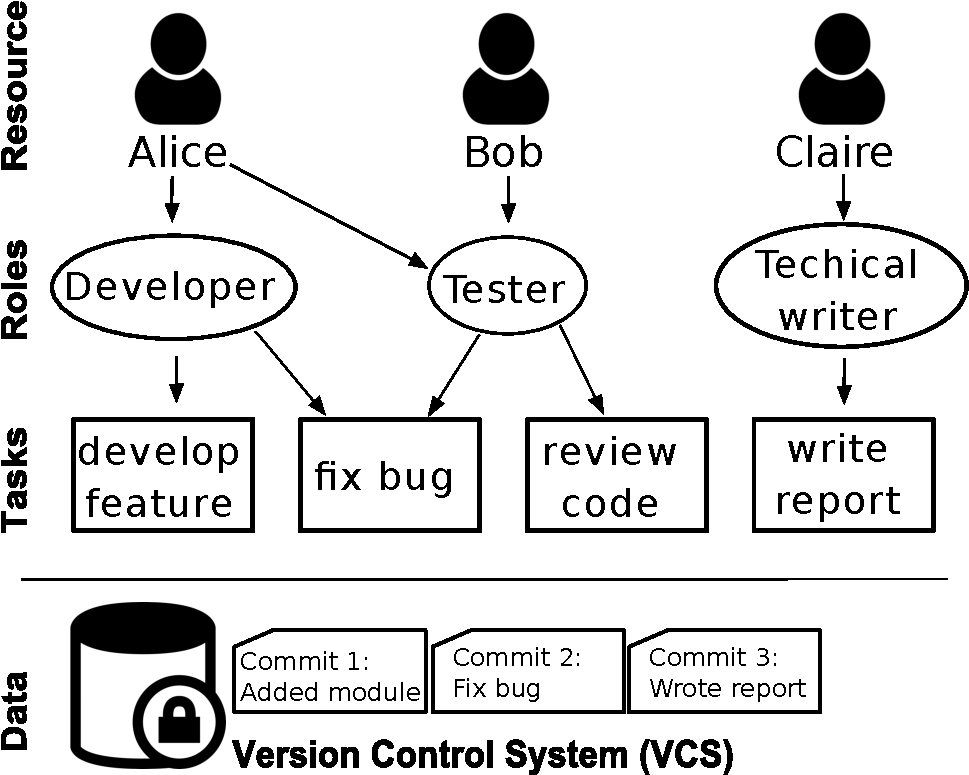
\includegraphics[width=.7\columnwidth]{ResourceClassification/figures/vcs3-crop.pdf}      
   \caption{Software project and resources}
   \label{fig:big-picture}
\end{figure}

\Gls*{vcs} logs provide rich and fine grained information about the changes in the project. 
A change may consist of a file being modified or new files being added to or removed from the repository. When changes are complete, it is possible to store them in the repository through a commit. Each commit contains a unique revision number, the identity of the resource who issued the commit, a timestamp, statistical information about the changes for each affected file, and a comment from the person who committed.

%A new commit moves forward the version of the files them were affected by the action of the user.
%Popular \glspl{vcs} are Git~\cite{torvalds2010git}, Mercurial~\cite{OSullivan2009} and SVN~\cite{pilato2008version}.

%Kushal's text
Let us consider the following example of how people use a \gls*{vcs} to collaborate in a project. Alice is a software engineer at Abc. ltd, and works on a project with her colleagues Bob and Claire. Alice is mainly assigned to the role \emph{developer}, but she can also be a \emph{tester}. Her tasks include the development of new features and fixing of related bugs. When a feature is ready she performs a commit and adds a new message where she describes her work, e.g. ``added new module to demo". At the same time she updates a file named ``rule''. This is reflected in the \gls{vcs} log, like in the first row of \Cref{tab:log-table-kushal}, identified by commit id 1. Bob is a \emph{tester} whose task is to ensure that the code submitted by Alice works properly. He discovers a bug in the ``setup'' interface file. Bob fixes those minor bugs and informs Alice of further work needed on the feature. Meanwhile, he commits his changes with commit id 2 and comments ``Modified the setup interface". Consequently, Alice reworks her code and commits a new version as reported in row 3 of \Cref{tab:log-table-kushal}, commenting her work with ``Update application interface". As a \emph{technical writer}, Claire takes over and starts to work on the documentation. She commits part of her work as in row 4. As the project continues, the work is accordingly stored in the log as in \Cref{tab:log-table-kushal}.

%\todo[inline]{\Cref{tab:log-table-kushal}: fill in with data from the running example}
%% Please add the following required packages to your document preamble:
% \usepackage{booktabs}
% \usepackage{multirow}
\begin{table}[]
\centering
\caption{Example of a \gls{vcs} log}
\vspace{5pt}
\label{tab:log-example}
\begin{tabular}{@{}cccll@{}}
   \toprule
   \textbf{ID}        & \textbf{Res}       & \textbf{Timestamp}                   & \textbf{Changelist} & \textbf{Comment}                                                                                 \\ \midrule
   \multirow{2}{*}{1} & \multirow{2}{*}{Y} & \multirow{2}{*}{2014-11-12 11:57:46} & A /file1            & \multirow{2}{*}{Added initial files}                                                             \\
   &                    &                                      & A /file2            &                                                                                                  \\ \midrule
   \multirow{2}{*}{2} & \multirow{2}{*}{X} & \multirow{2}{*}{2014-11-14 16:34:07} & M /file1            & \multirow{2}{*}{Developed interfaces}                                                            \\
   &                    &                                      & M /file2            &                                                                                                  \\ \midrule
   3                  & W                  & 2014-12-15 13:49:11                  & D /file1            & \begin{tabular}[c]{@{}l@{}}Reviewed interfaces. \\ Delete first. \\ Improve second.\end{tabular} \\ \midrule
   4                  & W                  & 2015-01-08 16:06:41                  & A /file3            & Added better interface                                                                           \\ \midrule
   \multirow{2}{*}{5} & \multirow{2}{*}{X} & \multirow{2}{*}{2015-01-13 11:47:09} & M /file2            & Improve backend                                                                                  \\
   &                    &                                      & M /file3            & Add feature                                                                                      \\ \midrule
   \multirow{2}{*}{6} & \multirow{2}{*}{Z} & \multirow{2}{*}{2015-01-16 16:50:29} & A /file4            & \multirow{2}{*}{Added tests}                                                                     \\
   &                    &                                      & A /file5            &                                                                                                  \\ \bottomrule
\end{tabular}
\end{table}
\begin{table*}[]
\centering
\caption{Example of a \glstext{vcs} log in the context of Organizational Perspective Discovery}
\label{tab:log-table-kushal}
   \begin{tabular}{m{0.5cm}m{1cm}m{3cm}m{2cm}m{4.5cm}}
%      \toprule
      \rot{\textbf{Commit ID}} & \rot{\textbf{User ID}} & \textbf{TimeStamp}  & \textbf{Updated Files}                                        & \textbf{Comment}                                         \\ \midrule
      1                  & Alice            & 2014-10-12 13:29:09 & \begin{tabular}[c]{@{}l@{}}Demo.java\\ rule.txt\end{tabular}   & Added new module to demo and updated rules               \\
      2                  & Bob              & 2014-11-01 18:16:52 & Setup.exe                                                     & Modified the setup interface                             \\
      3                  & Alice            & 2015-06-14 09:13:14 & Demo.java                                                      & Update the application interface                         \\
      4                  & Claire           & 2015-07-12 15:05:43 & \begin{tabular}[c]{@{}l@{}}graph.svg \\ todo.doc\end{tabular} & Define initial process diagram \& listed remaining tasks \\
      \ldots                  & \ldots              & \ldots & \ldots                                                     & \ldots                                                  \\ 
%      \bottomrule
   \end{tabular}
\end{table*}

As we can see from the example, user work is tracked in a fine granular way by the \gls{vcs}. The challenge is to use log information for getting insights into the roles of project members. The following section discusses related literature that has addressed role discovery.

%\subsection{Version Control Systems}
%
%A VCS is an application with the purpose of tracking changes in documents. The most common example of such a document is source code of software, but it can also be natural language text, structured text content or any other kind of information. Each change of a file creates a new version or revision of this file.
%
%
%All versions are stored in a repository and can be accessed for different purposes, for example to switch to an older version, to find out which user made a certain change or to revert the document to a previous state. A commit is a collection of file changes passed to the VCS at once by a single user. Usually users provide a message for each commit, which describes the contributed changes. A VCS log is a chronological history of commits. The information included in these logs depends on the VCS and can be configured. It usually includes for each commit some kind of identifier, the author, a timestamp, the commit message and the number of added, modified and deleted files. The most commonly used systems for software development are Git~\cite{torvalds2010git}, Mercurial~\cite{OSullivan2009} and SVN~\cite{pilato2008version}.
%
%
%Version control systems can be used within companies to enable the individual employees to work together on projects. Tasks are distributed and the results then have to be merged to create the product. This can be done via commits in a VCS. It documents the current status of the project and changes have to be committed into the repository. Conflicts, due to multiple users working on the same resource, have to be resolved and the VCS creates a history, where every change can be tracked. Additionally, the users can try out their ideas on their own systems without breaking the whole project.
%
%
%The VCS also keeps a history of all versions. Customers receive a certain product version and for bug fixes for this specific version only the version id is required, instead of maintaining a copy for each customer. For open source projects it enables users to work around the world at any time, while enabling new workflows. Additionally, the entry barrier for new users is lowered. Downloading the repository, applying changes and committing them, even if he /she only once advances the project, can be done by anyone. 
%
%
%\subsection{User Classes}
%
%There are various types of user classes. The most apparent interpretation are classes corresponding to typical official or implicit roles within a software project (e.g. developer, tester...). But there are also other possible ways of classification, such as by individual experience, age of users, distinction in supervisor, subordinate relationships commitment, commitment and various demographics or personality traits. This research focuses on the project roles but additional classifications are not excluded.
%
%There is a large number of roles in software development
%
%proposed and analyzed by literature. Roles relevant for this context have to be identified, meaning that these roles create commits at all and that they provide some kind of characteristics to identify them. The identified roles which fulfill these conditions are: developer (can be split up into backend, frontend or web developers), tester, designer, technical writer, architect, toolsmith, database expert and (VCS or build) administrator (Acua \& Juristo, 2004) (Shore, 2007).
%
%However, especially in smaller teams and projects it is quite common that a single user has multiple roles.  In some cases these roles are formally defined, in others they are just reflected by the tasks and responsibilities of the user. Especially in open source projects there is often no explicit separation of roles.

%\subsection{Requirements}

As mentioned in the previous section, the focus of this section lies on mining and analyzing properties of the users of \gls{vcs}. Users belong to preset classes and they commit message styles. Based on this assumption, the following requirements are defined.

\begin{itemize} %\IEEEsetlabelwidth{Z}
      
\item[\textbf{RQ1. Cluster users from event log.}] 
We want to provide a classification of the users of a \gls{vcs} by using the information contained in the log files. Comment messages and other data must be investigated for useful features. The classification must separate the users into clusters, and the most expressive features and their combinations must be identified.  These clusters can then be further analyzed by means of the next research question.

\item[\textbf{RQ2. Create user profiles.}]
Based on the created clusters, meaningful classes should be derived. The chosen features influence the types of classes that can be created. These classes must present an intelligible distinction among each other. This requirement aims at making class distinctions clear-cut. Moreover, it aims at creating profiles for the class members reflecting behavior, based on the analyzed features.

\item[\textbf{RQ3. Generalize approach.}]
The last research question examines the differences among the created classes in detail. It compares the results from different log files and identifies the reasons for dissimilarities. Therefore, it evaluates the quality of the classification and its applicability for different version control systems.

\end{itemize}


\subsection{Related Work}
Role discovery has been addressed by literature in different settings and from several points of view. Here we highlight existing efforts from a data perspective.

\subsubsection{Structured data approaches}
This class of methods includes algorithms that make use of quantifiable data. We divide them into: 
\begin{inparaenum}[\itshape a)]
   \item \gls*{msr} approaches; and
   \item \gls*{pm} approaches.
\end{inparaenum}

\paragraph{\bfseries Mining software repositories approaches}
In the area of \gls*{msr}, \cite{Yu.LiguoRamaswamy.2007} use a hierarchical clustering based on user interactions to identify two categories of users: \emph{core member} and \emph{associate member}. Core members are those users whose interaction frequency is higher than a given threshold. Associate members are instead users whose interaction frequency is below the threshold.
\cite{Alonso2008} use a rule-based classifier that maps file types onto categories and hence each author who modified a file is linked to the files' category. ~\cite{gousios2008measuring} classify developers contribution based on \gls*{loc} changes and infer activities from them. \cite{Begel2010} developed the Codebook software tool a utility for finding experts. They use a social network approach that combines sources from people, artifacts, and textual references to other people. 
%Codebook is able to crawl several repositories and store the data as a graph in a database. Using a social network approach, that combines sources from people, artifacts, and as well as textual allusions to other people, this tool allows for finding experts. 
\cite{Ying2014} study developer profiles in terms of their interaction with the software artifacts to understand how they modify files and to further recommend changes based on history from \gls*{vcs} logs. \cite{Fuller2014a} investigate user roles in innovation-contest communities. They use quantitative methods to analyze user activity logs and interpretative to categorize qualitative comments into classes. 
%Furthermore, they used clustering to identify six user types: master, idea generator, socializer, efficient contributor, passive idea generator, passive commentator. Their work point out that different users are indeed characterized by behavioral contribution patterns. 

\paragraph{\bfseries Process mining approaches}
Efforts have been done to analyze software repositories with process mining techniques. \cite{rubin2007process} implement a multi-perspective incremental mining that is able to continuously integrate sources of evidence and improve the software engineering process as the user interacts with the documents in the repository. Their approach allows for mining other perspectives, such as roles, by applying social network analysis. However, only statistical methods can be applied to their output, since it lacks the comments that are associated to file changes. In the same setting, \cite{DBLP:conf/csmr/PoncinSB11} developed \textsc{frasr}, a framework for analyzing software repositories. \textsc{frasr} can be used in order to transform \gls*{vcs} logs data into the XES~\citep{verbeek2010xes} data format that can be further analyzed with process mining tools like ProM\footnote{http://www.promtools.org/doku.php}. 
\cite{Song2008} focus on three types of organizational mining 
\begin{inparaenum}[\itshape i)]
   \item organizational model mining, 
   \item social network analysis, and 
   \item information flows between organizational entities.
\end{inparaenum} 
\cite{Schonig2015} propose a mining technique to discover resource-aware declarative processes.

\subsubsection{Unstructured data} \cite{Maalej2010} use \gls*{nlp} for automating descriptions of work sessions by analyzing developers' informal text notes about their tasks. Developers are then classified into two classes based on their behavior: developers who use problem information to refer to their current activity and developers who refer to task and requirements. \cite{Kouters2012} developed an identity merging algorithm based on Latent Semantic Analysis (LSA) to disambiguate user emails. \cite{Licorish2014} mined developer comments to understand their attitudes.

\subsubsection{Other related work} The term \emph{role mining} often points to role mining algorithms based on \gls*{rbac} systems. These algorithms take as input predefined roles that are given as a matrix, where each user is assigned to access permissions. A number of algorithms have been developed to mine roles from \gls*{rbac} systems alone \citep{Lu2015,frank2013role} or combining their data with process history logs, as in \citep{baumgrass2012deriving}. A survey of existing techniques and algorithms can be found in \citep{Mitra2016}. Our work is disjoint from this class of algorithms as \gls*{vcs} does not contain access control information. 
\cite{Bhattacharya2014} propose a contributor graph-based model. By constructing a source-based profile, and a bug-based profile, they are able to identify seven roles: \emph{patch tester}, \emph{assist}, \emph{triager}, \emph{bug analyst}, \emph{core developer}, \emph{bug fixer}, and \emph{patch-quality improver}. \cite{hoda2013self} use a \gls*{gt} approach to study agile teams. Their work distinguishes the roles of \emph{mentor}, \emph{coordinator}, \emph{translator}, \emph{champion}, \emph{promoter}, and \emph{terminator}.


This work builds upon existing literature in that it strives to get insights on organizational level like in \cite{rubin2007process} and \cite{Song2008}, but it takes into account unstructured data. Differently from the literature that works with unstructured data, we explicitly consider the problem of role discovery, i.e. label resources with roles. Lastly, this approach differs from \cite{Bhattacharya2014} and \cite{hoda2013self} since we further adopt \gls*{nlp} techniques.


\section{Solution Concept}\label{sec:concept}

%Commit messages contain metadata and content. For analysis of users and roles both parts are important. Metadata includes the author, which is essential for gaining a unique identifier of the committer. The content gives some indications on roles. Data needs to be cleaned. Changed roles, one time committers, or several identities for the same use, are some of the challenges that need to be handled. 

Commits contain fine grained information about many aspects of a work unit. We are interested in three aspects. First we consider distinct identities and timestamps of commits. This makes it possible to compute how frequent and how distant in time commits appear in a project. Second, we obtain information about the authors. Authors are explicitly stated in the commit. Third, we consider their comments. Comments are written in natural language and need to be parsed and preprocessed before we can use them.

Once data is preprocessed, the analysis can start with a direct approach of connecting one commit message to one user and to the corresponding role. In this approach user roles are linked to the authors of commits. However, roles are not always available a priori. In these cases, a commit-based approach can be adopted. This method operates on the commits and assigns types to them first. Further analysis then maps these types to possible user roles. This approach is not a direct mapping. Instead, it allows for more flexible role discovery. We use this approach to also predict roles, based on user profiles that we create from the commit types.

\begin{figure}[htb]
   \centering
   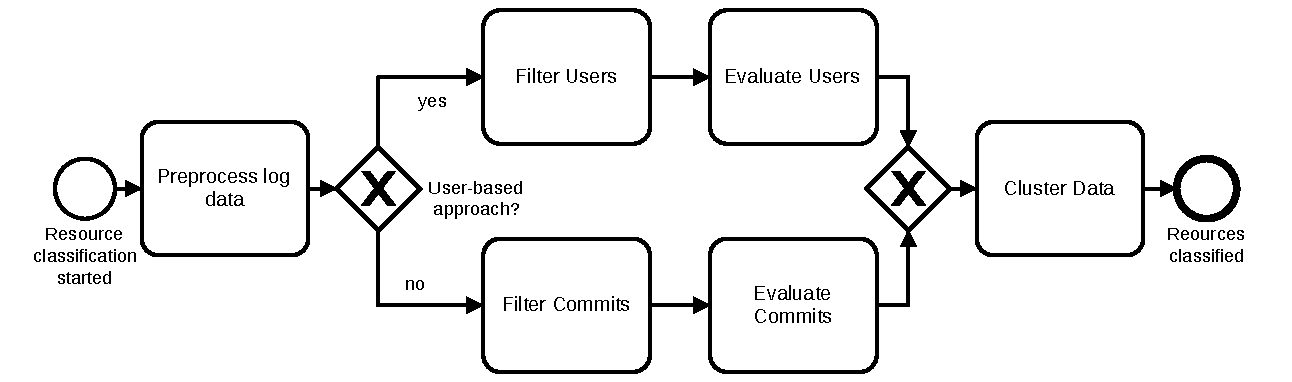
\includegraphics[width=1\linewidth]{ResourceClassification/figures/approach-bpmn}
   \caption[Approach to role classification from VCS logs]{Approach to role classification from VCS logs}
   \label{fig:approach-bpmn}
\end{figure}

\Cref{fig:approach-bpmn} illustrates the steps of our approach through a BPMN diagram. In the first step we preprocess the data and parse the SVN log file. Then we account for two different types of classification: user-based and commit-based. These approaches require a prior step where we filter the data according to users or to commits. Both approaches include an evaluation step where we map keywords and information on file types to users or commits, respectively. The last step is the data classification. \Cref{sec:impl} describes both approaches in detail.

\subsection{Implementation}
\label{sec:impl}

We implemented the outlined solution concept in a Python script. This script automatically fetches, processes and analyses the log files and creates a classification model that is based on the extracted information. The following tools are used for implementation:

\begin{description}

\item[\textbf{Technology.}] Python is a general-purpose, high-level programming language. It is open source, easy to use and offers various third party modules\footnote{https://www.python.org/}.

\item[\textbf{Machine Learning.}] The Scikit Learn module is used for machine learning\footnote{http://scikit-learn.org/stable/}. We used \glspl*{dt} for classification and regression. \Glspl*{dt} are a supervised learning method whose goal is to create a model that predicts a target feature of variable by inferring existing rules from the data.

\item[\textbf{Natural Language Processing.}] The Natural Language Toolkit (NTLK) offers methods to extract additional information from everyday communication. Among others, we rely on the \emph{bag of words} technique that analyzes word occurrences\footnote{http://www.nltk.org/book/ch00.html}.

\end{description}

Next, we discuss the data selection criteria. While there are many accessible code repositories, picking a dataset of appropriate size and quality proves to be rather challenging. We need to consider:

\begin{description}

\item[\textbf{Diversity}.] Classification on a single repository might not produce a generally applicable result, whereas using more repositories increases complexity.

\item[\textbf{Size}.] Individual repositories' size is determined by the number of commits.

\item[\textbf{Roles}.] The real roles of the contributors of a repository is required for certain classification steps and the verification of results.

\item[\textbf{Type}.] Differences in organizational aspects of the projects: the type of the development team (e.g. professional or hobby), type of software (e.g. proprietary or open-source), and type of platform (e.g. private server or public repository hosting service) can influence the way repositories are used.

\item[\textbf{Backend}.] There exists a plethora of version control systems, each with their unique characteristics and formats. The approach should be able to handle popular systems including Subversion (SVN), Git, and Mercurial.

\end{description}

Based on these criteria, we selected three repositories for analysis, each with thousands of commits:

\begin{enumerate}

\item Main code repository of the company Infinica. Proprietary software. VCS: Mercurial

\item ProM Sourceforge project repository. Open source software. VCS: SVN

\item Camunda GitHub project repository. Open source software. VCS: Git

\end{enumerate}


These repositories cover a broad range of the above mentioned differences. The necessary role information was reviewed by interviews with the main contributors of these projects. While two repositories were openly available, the third was granted a direct access from within the company.

%First of all, browsing through the commit messages created an understanding of the structure of the log files, the type of information available for extraction and the way VCS commits are typically used in the different projects. They contain the most useful information but are also the least predictable factor, because there are no general rules on how to formulate such a message. 

An initial screening of commit messages in the repositories revealed that there is useful information within most of the messages, but the variance regarding the style and content of the messages is high between commits and users.
From the messages, certain words and phrases can be extracted, which can be linked to a specific class. In a next step, the log files were preprocessed removing commits and/or users with faulty information, merging users with several accounts and anonymizing the data if required. 

%The first step of creating the algorithm, once the log files were obtained and their basic structure was known, is to transform them into a common in-memory object model. 
To unify the different systems, we create a shared object model to store the relevant information.
%Three different functions, providing the same output for different input formats, were required to cover all three systems (Git, Svn, Mercurial). 
This model consists of a commit object for each commit in the log, consisting of an id, an author, a message, a timestamp and lists of all added, modified and deleted files. From this model it is possible to derive a second model consisting of the users, by aggregating the information for each author name occurring in the commits.

In the following, we present two ways to tackle the problem of classification of users into their respective roles. First, the \emph{user-based} approach focuses on the users at an aggregated level. Second, the \emph{commit-based} approach classifies individual commits to allow for a finer grained classification. 

%For further analysis and classification steps, efforts have been split up into two approaches. The first one focuses purely on the users and the features deductible for them. We soon realized though that this method, while providing some promising insights, had certain limitations and left out some potentially valuable information. Therefore a second approach was incorporated taking a closer look at the individual commits. The two approaches are outlined in more detail in the following sections.

\subsection{User-based Approach}

The main idea of this approach is to use clustering in order to find potential user classes and build a classification model based on those clusters, which represent a comprehensible, existing class of users. As a clustering method we used k-means.

The first step is feature selection. We identified the following features per user.

\begin{itemize}

\item Total number of commits.

\item Timeframe: the time between the first and last commit of the user (approximates the time a user has been working on a project).

\item Commit frequency: total number of commits divided by the time frame. Represents the number of commits a user makes within a certain period of time (e.g. day, month).

\item Commit message length: average length of commit messages in number of words.

\item Keyword occurrence: how often a certain word (e.g. "test", "fix") is used relative to the total number of words.

\item Number of added/modified/deleted files.

\item Affected file types: how often a file with a certain format (e.g. .java, .html) are modified by a user, relative to the total number of modified files.

\end{itemize}


%In order to find useful clusters, an experimentation with different combinations of features is necessary. For each of these combinations the optimal cluster number has to be found. While the clustering and optimizing tasks can be automated, the clusters have to be evaluated manually. This makes it impossible to test all possible combinations of features, especially when including the keyword occurrence numbers, as the list of keywords with potential value was far too large. Combinations that promise useful results are selected. Evaluation is done using plots as well as looking at the raw data to find connections between the identified clusters and the existing classes in the sample data.


From the clusters generated with this method, classification models are built using the decision tree method. This method uses tree graphs for representing the model. Each branching in the tree represents one decision based on the characteristics of a certain data point. Each leaf of the tree stands for a class. The classification is done by going through the tree for each data point and assigning it the class of the leaf it reaches. The models are trained for the three data sets individually. For verification of their quality, the models are cross validated with the other data sets respectively.


\subsection{Commit-based Approach}

There are multiple reasons for exploring a second approach in addition to the user clustering. As already mentioned above, the research led to the conclusion that in many cases a user can have multiple roles or execute many tasks not belonging to her primary role. This kind of use case is hard to cover using only the simple clustering method. Another reason is that a lot of information is lost when aggregating the commit information for users. This leads to the idea of classifying individual commits.


The algorithm iterates over commits and tries to assign types to them. The types are assigned based on the analysis of the commit message, and on the file extensions. The commit message is searched for certain keywords and phrases which are connected to types. The file extensions are searched for known file types fitting to a commit type. There are certain overlaps between commit types, for example the type addition can be a development or test commit. In those cases where one identified type is a more specific description for another, only the more specific one is included into the further analysis. The identified commits and the related keywords and file types are listed in \Cref{tab:keywords}.

\begin{table}[]
   \centering
   \caption{Keyword lemmas used for classification}
   \label{tab:keywords}
   \begin{tabular}{@{}m{.2\columnwidth}m{.7\columnwidth}@{}}
      \toprule
      \textbf{Class} & \textbf{Keywords}                                                                                               \\ \midrule
      Test           & test testcase test case unittest unit test integrationtest fitnesstest fitness test                                     \\
      Development    & implement improve update script                                                                                 \\
      Web            & web spring http http rest html css servlet                                                                      \\
      Backend        & engine                                                                                                          \\
      Maintenance    & bugfix fix patch cleanup clean up clean                                                                         \\
      Refactor       & refactor rename move revert                                                                                     \\
      Documentation  & document javadoc readme userguide guide tutorial faq translate doc i18n *.txt *.doc *.docx *.text *.tex *.pdf \\
      Design         & style icon font layout *.png *.svg *.jpg                                                                        \\
      Build          & build compile release                                                                                           \\
      Data           & data database sql postgre postgresql                                                                            \\
      Tool           & tool library framework depend upgrade                                                                           \\
      Addition       & add new create                                                                                                  \\
      Removal        & delete remove                                                                                                   \\
      vcsManagement  & svn git mercurial                                                                                               \\
      Automated      & automated release, automated nightly                                                                            \\
      Merge          & merge                                                                                                           \\ \bottomrule
   \end{tabular}
\end{table}

After assigning the commit types, the commits can be aggregated for the individual users resulting in the absolute occurrence numbers of each type for each user. Dividing each of these values by the total number of commits of the user, we get percentages for each type. These percentages tell how the work of a user is distributed among the different kinds of tasks which appear in a VCS. These user profiles are a form of classification, which is not as simple and concise as assigning one definite class for each user, but has the advantage of covering secondary roles and minor tasks. They can be useful for analyzing smaller project teams with multiple roles for one user.

The classification task is done on user profiles. A table of user profiles is created and a role for each user manually inserted, based on the role information of the data sets. For this part the Infinica data set is used, because it is the one with the most extensive information base and it has the most diverse and comprehensive set of roles among the shosen repositories. Four roles are assigned to the Infinica users: Web developers, other developers, testers and support. The last one is an aggregation of users who have different official roles but contribute in the VCS mainly in form of minor, supportive tasks.

The classification task was done in two ways: 1. Manual analysis of the table and derivation of rules by looking for similarities between users with the same role. 2. Automated classification in line with our original concept. For the latter the decision tree method is used. In this case the commit type percentages are used as features and the manually assigned roles as classes. The resulting decision tree model was validated against the ProM and Camunda data sets.


The final algorithm including retrieval, processing and analysis of data as well as classification and verification, consists of roughly 700 lines of code. The results for the two approaches are discussed below.


\section{Evaluation}

In the first step of the user-based approach, the most expressive features of the Infinica data set were identified. The solution was tested on the Infinica data set due to the immediate availability of detailed information about the log file. The best results were achieved with the combination of the commit frequency and the occurrence numbers of test related keywords.


The commit frequency is a strong indicator of developers. Moreover, it also differentiates between the working preferences of the developers. The group with the lower frequencies tends to work locally on their machines and pushes their work when it is finished. Whereas, the developer group frequently pushes incremental changes to the repository, so that everybody is updated and works with the latest code.


Test-related keywords can not only identify testers, but also differentiate between their expertise. The sum of the words "test", "tested", "testing", "tests" suffices to make a distinction between testers and developers. Additionally, manual testers use these words less often than their technical counterparts, who are more focused on automation.


The first part of the commit-based algorithm implementation, i.e., the commit classification, was successfully tested on all three data sets combined. For all three sets we achieved a similar coverage (percentage of commits which could be assigned some type). For Infinica the coverage was 88,94\%, for Camunda it was 90,25\% and for ProM 86,65\%.

While the user profiles were originally intended as an intermediary step and a means to verify and improve the quality of our approach, they proved to be a useful perspective on user roles, beyond the simple categorisation using a single class. Especially when using a graphical representation such as the pie charts which can be seen in \Cref{fig:developer} and \Cref{fig:tester}, the commit distribution provides an interesting insight in the actual roles and tasks of users.

\begin{figure*}[ht]
   \centering
   \begin{subfigure}[t]{.5\textwidth}
      \centering
      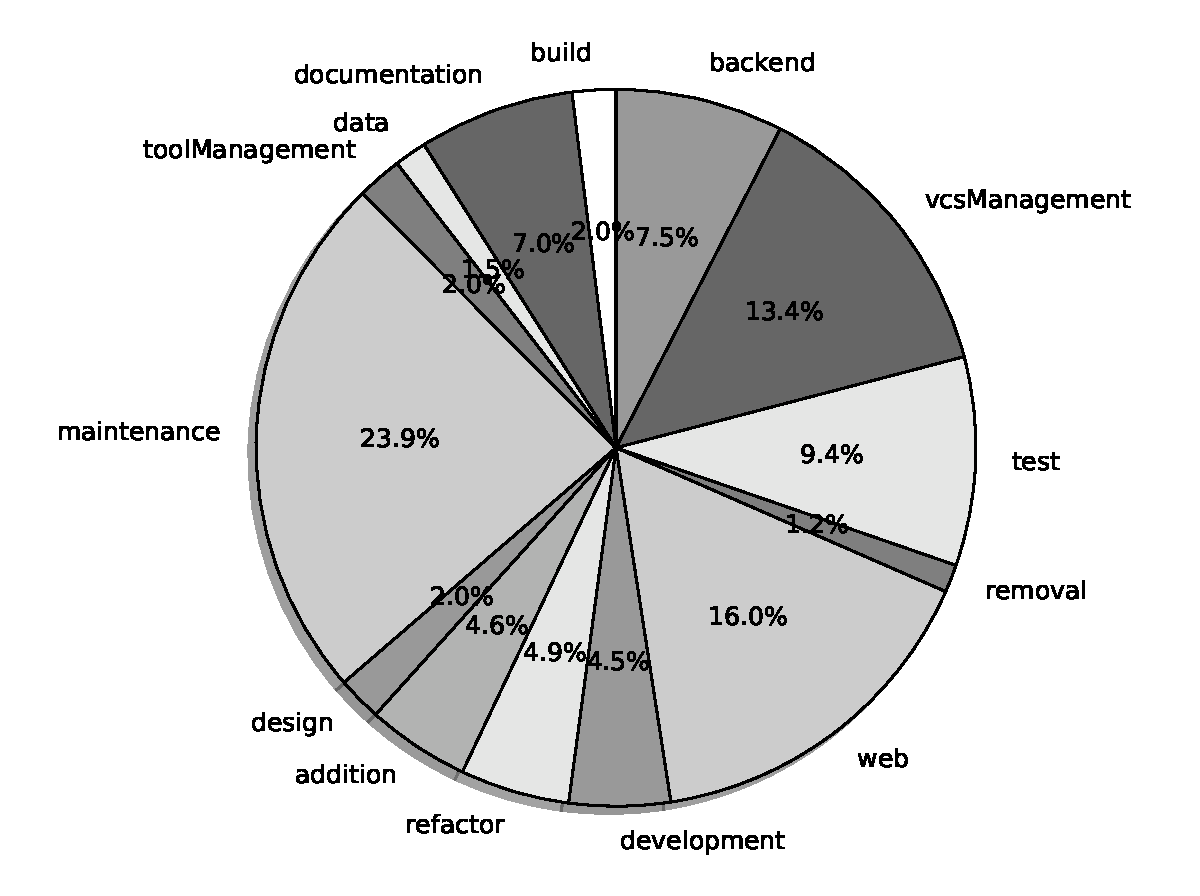
\includegraphics[width=\linewidth]{ResourceClassification/figures/infinica_developer.pdf}
      \caption{User profile for a backend developer}
      \label{fig:developer} 
   \end{subfigure}%
   \begin{subfigure}[t]{.5\textwidth}
      \centering
      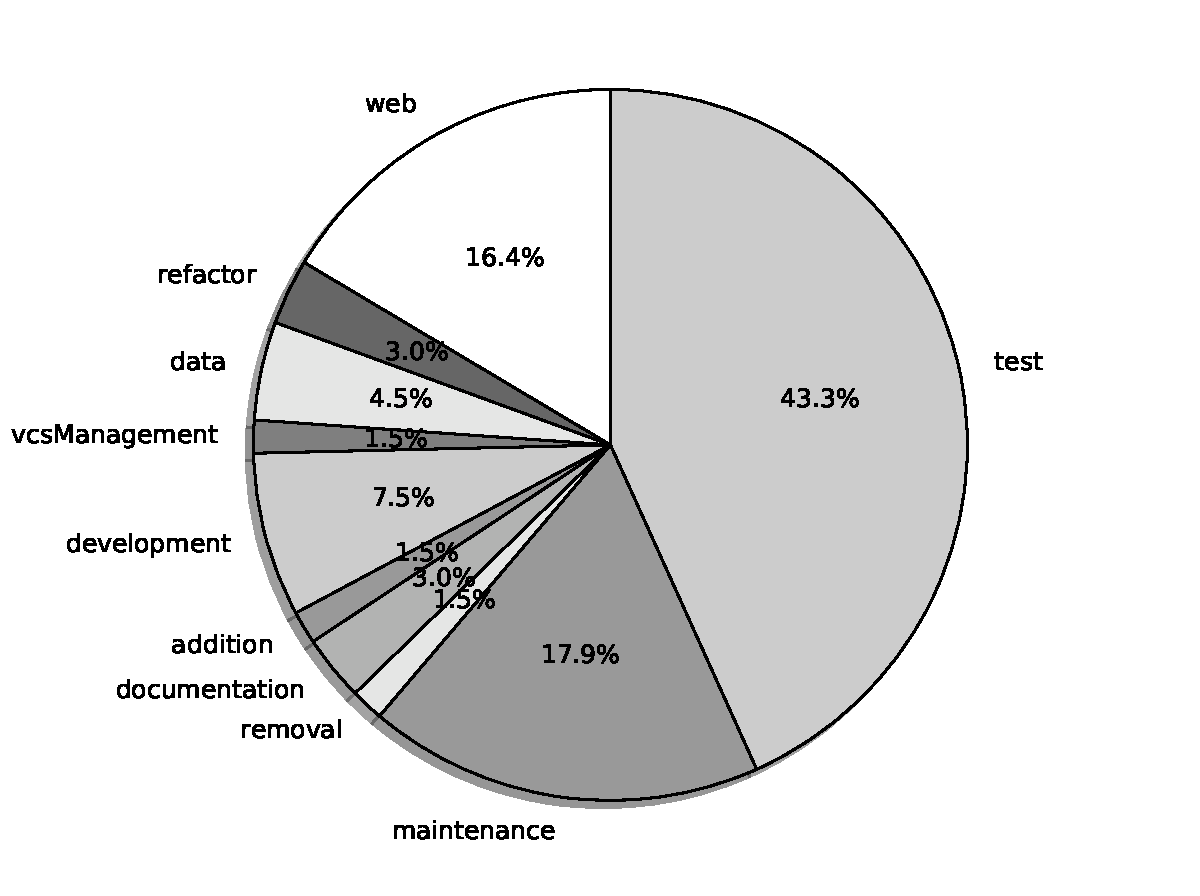
\includegraphics[width=\linewidth]{ResourceClassification/figures/infinica_tester.pdf}
      \caption{User profile for a tester}
      \label{fig:tester} 
   \end{subfigure}
   \caption{Commit distributions of the Infinica dataset}
   \label{fig:test}
\end{figure*}

\begin{figure}[h]
	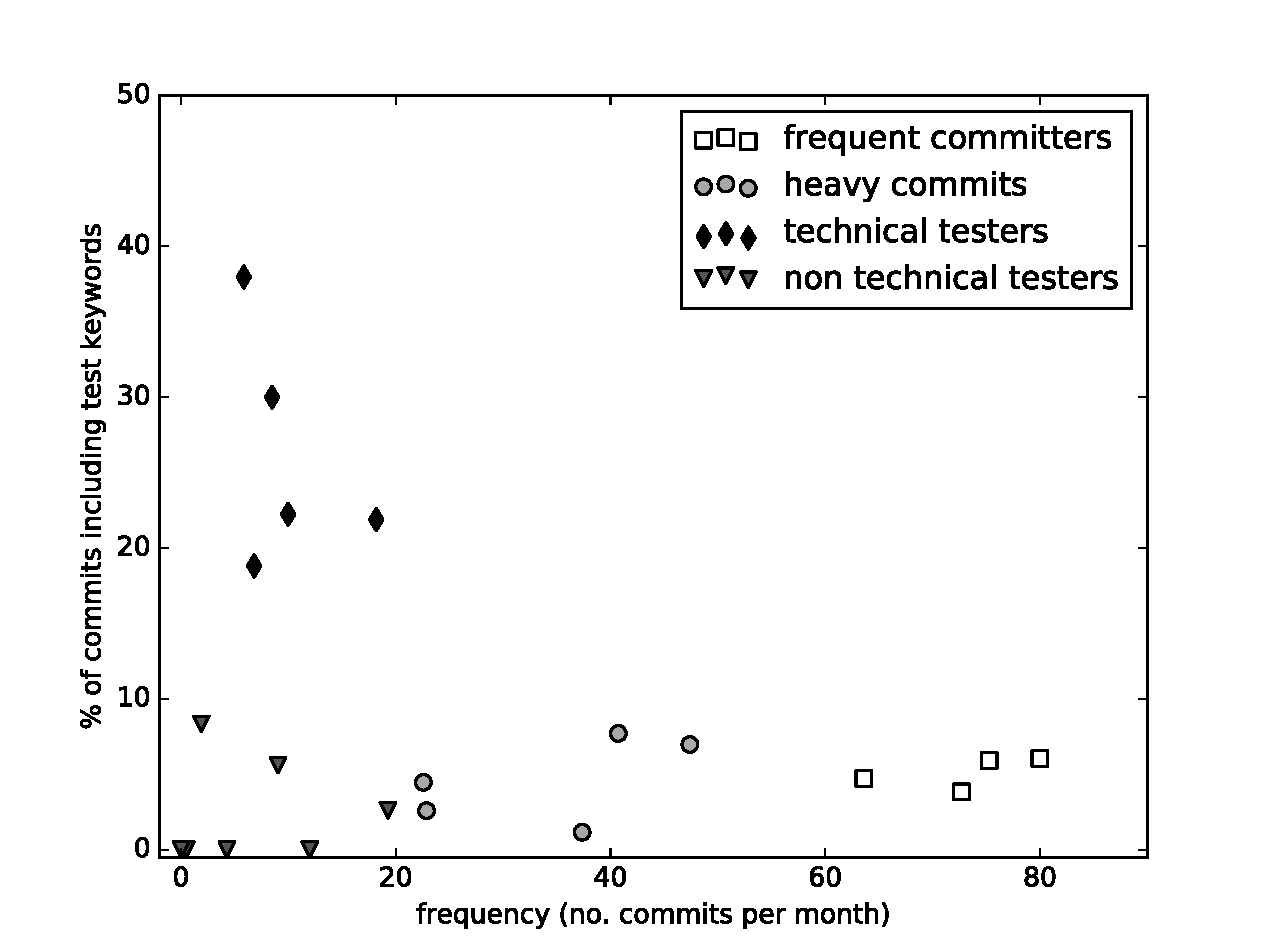
\includegraphics[width=\columnwidth]{ResourceClassification/figures/infinica4k_black.pdf}
	\caption{Scatterplot with highlighted clusters (k=4) based on the Infinica data set.}
	\label{fig:infinica4k}
\end{figure}

The Infinica dataset is divided successfully into expressive classes with k-means clustering with a k=4 shown in \Cref{fig:infinica4k}. The developers (light grey circle and white square) are split off based on their higher frequency in the first step of the decision tree and the following classes are derived:

\begin{itemize}

\item \textbf{Developers - frequent committers:} The square cluster is comprised  of developers which push every change to the repository.

\item \textbf{Developers - heavy commits:} The circle cluster contains developers who work on their local machine and push less frequently. However, they have bigger commits containing more changes.

\item \textbf{Testers - technical:} Testers focused on automating the testing process are in the diamond cluster. They are solely senior developers but not all of them are situated in this group.

\item \textbf{Testers - non technical:} The triangle cluster is comprised of less technical testers which tend to do more manual testing. Additionally, it includes the professional services team.

\end{itemize}

\Cref{tab:user-profiles2} shows an excerpt of the user profiles and role assignments for the Infinica data set. The commit types development, backend, maintenance and refactor have been merged to a single type development, as the other, more specific types provided no additional value in this case. Also the types "addition", "removal" and "merge" have been omitted due to a lack of semantic meaning. The data visible in the table was used for the manual classification as well as the creation of the decision tree model.

% Please add the following required packages to your document preamble:
% \usepackage{booktabs}
\begin{table*}[]
   \centering
   \caption{Excerpt from user profiles with roles for Infinica data set}
   \label{tab:user-profiles2}
   \begin{tabular}{@{}rrrrrrrrrc@{}}
      \toprule
      \multicolumn{1}{c}{\textbf{\begin{tabular}[c]{@{}c@{}}test \\ \%\end{tabular}}} & \multicolumn{1}{c}{\textbf{\begin{tabular}[c]{@{}c@{}}development \\ \%\end{tabular}}} & \multicolumn{1}{c}{\textbf{\begin{tabular}[c]{@{}c@{}}web \\ \%\end{tabular}}} & \multicolumn{1}{c}{\textbf{\begin{tabular}[c]{@{}c@{}}documentation \\ \%\end{tabular}}} & \multicolumn{1}{c}{\textbf{\begin{tabular}[c]{@{}c@{}}vcsManagement \\ \%\end{tabular}}} & \multicolumn{1}{c}{\textbf{\begin{tabular}[c]{@{}c@{}}build\\ \%\end{tabular}}} & \multicolumn{1}{c}{\textbf{\begin{tabular}[c]{@{}c@{}}toolManagement\\ \%\end{tabular}}} & \multicolumn{1}{c}{\textbf{\begin{tabular}[c]{@{}c@{}}data\\ \%\end{tabular}}} & \multicolumn{1}{c}{\textbf{\begin{tabular}[c]{@{}c@{}}design\\ \%\end{tabular}}} & \textbf{\begin{tabular}[c]{@{}c@{}}class\\ name\end{tabular}} \\ \midrule
      6.07                                                                            & 39.49                                                                                  & 26.40                                                                          & 7.94                                                                                     & 0.23                                                                                     & 3.27                                                                            & 0.70                                                                                     & 0.23                                                                           & 11.21                                                                            & dev                                                           \\
      9.41                                                                            & 40.90                                                                                  & 15.99                                                                          & 7.00                                                                                     & 13.37                                                                                    & 1.96                                                                            & 2.04                                                                                     & 1.46                                                                           & 2.00                                                                             & dev                                                           \\
      3.83                                                                            & 26.78                                                                                  & 44.70                                                                          & 2.90                                                                                     & 4.70                                                                                     & 3.93                                                                            & 0.60                                                                                     & 2.95                                                                           & 6.01                                                                             & webdev                                                        \\
      0.00                                                                            & 28.07                                                                                  & 52.28                                                                          & 2.46                                                                                     & 0.00                                                                                     & 5.26                                                                            & 1.40                                                                                     & 0.35                                                                           & 8.42                                                                             & webdev                                                        \\
      43.28                                                                           & 28.36                                                                                  & 16.42                                                                          & 2.99                                                                                     & 1.49                                                                                     & 0.00                                                                            & 0.00                                                                                     & 4.48                                                                           & 0.00                                                                             & tester                                                        \\
      23.99                                                                           & 27.73                                                                                  & 15.26                                                                          & 7.79                                                                                     & 0.00                                                                                     & 2.49                                                                            & 1.56                                                                                     & 1.25                                                                           & 4.67                                                                             & tester                                                        \\
      0.00                                                                            & 7.94                                                                                   & 38.10                                                                          & 0.00                                                                                     & 38.10                                                                                    & 1.59                                                                            & 4.76                                                                                     & 0.00                                                                           & 9.52                                                                             & support                                                       \\
      1.19                                                                            & 3.39                                                                                   & 46.15                                                                          & 1.61                                                                                     & 46.15                                                                                    & 0.08                                                                            & 0.17                                                                                     & 1.19                                                                           & 0.08                                                                             & support                                                       \\
      ...                                                                             & ...                                                                                    & ...                                                                            & ...                                                                                      & ...                                                                                      & ...                                                                             & ...                                                                                      & ...                                                                            & ...                                                                              & \multicolumn{1}{r}{...}                                       \\ \bottomrule
   \end{tabular}
\end{table*}

We identified 4 role-based classes which were visible from the Infinica data. Those were testers, with more than 20\% of their commits being of type test and between 30\% and 50\% of type development, developers with above 50\% development commits, web developers with more than 40\% of type web, and 20\% of other development and non-technical users with less than 20\% development. In addition to those, we found some less obvious hints for additional classes, represented by minor, secondary roles of users. These were not represented as actual existing roles in our data, so we could not verify our assumptions. The corresponding classes we suggest for those are technical writer with more than 40\% documentation commits, designers with above 30\% design commits, users with various administration tasks, represented by high numbers of the types build, vcsManagment and toolManagement and database experts with a large percentage of data commits.

When applying the optimal features and clusters deduced from the Infinica data set on the ProM data set, different but still meaningful user classes are derived. This is due to the fact that the Infinica data set represents the development process within a company, whereas ProM is an academic project where researchers continuously join and leave. However, it still required to get invited for working on the project which creates an entry barrier. All members are developers without any designated testers. The ProM data set can be divided into the following four classes as shown in \Cref{fig:prom4k}.

\begin{itemize}
\item \textbf{Core developers:} The employed users of the ProM project are situated in the square cluster. Their commit frequency and absolute number of commits is far above the others. There is also a system user in this class. Its main task is building the project.

\item \textbf{Engaged developers:} The circle cluster contains developers which also write tests. They are more committed and they put more effort into the development.

\item \textbf{One-time developers:} The enagement of this group ends with the addition of their required functionality. The majority of the users falls into this class and it is represented by the diamond cluster.

\item \textbf{Testers:} Despite the lack of testers in the ProM data set two have been identified as such in the triangle cluster.
\end{itemize}


\begin{figure}
   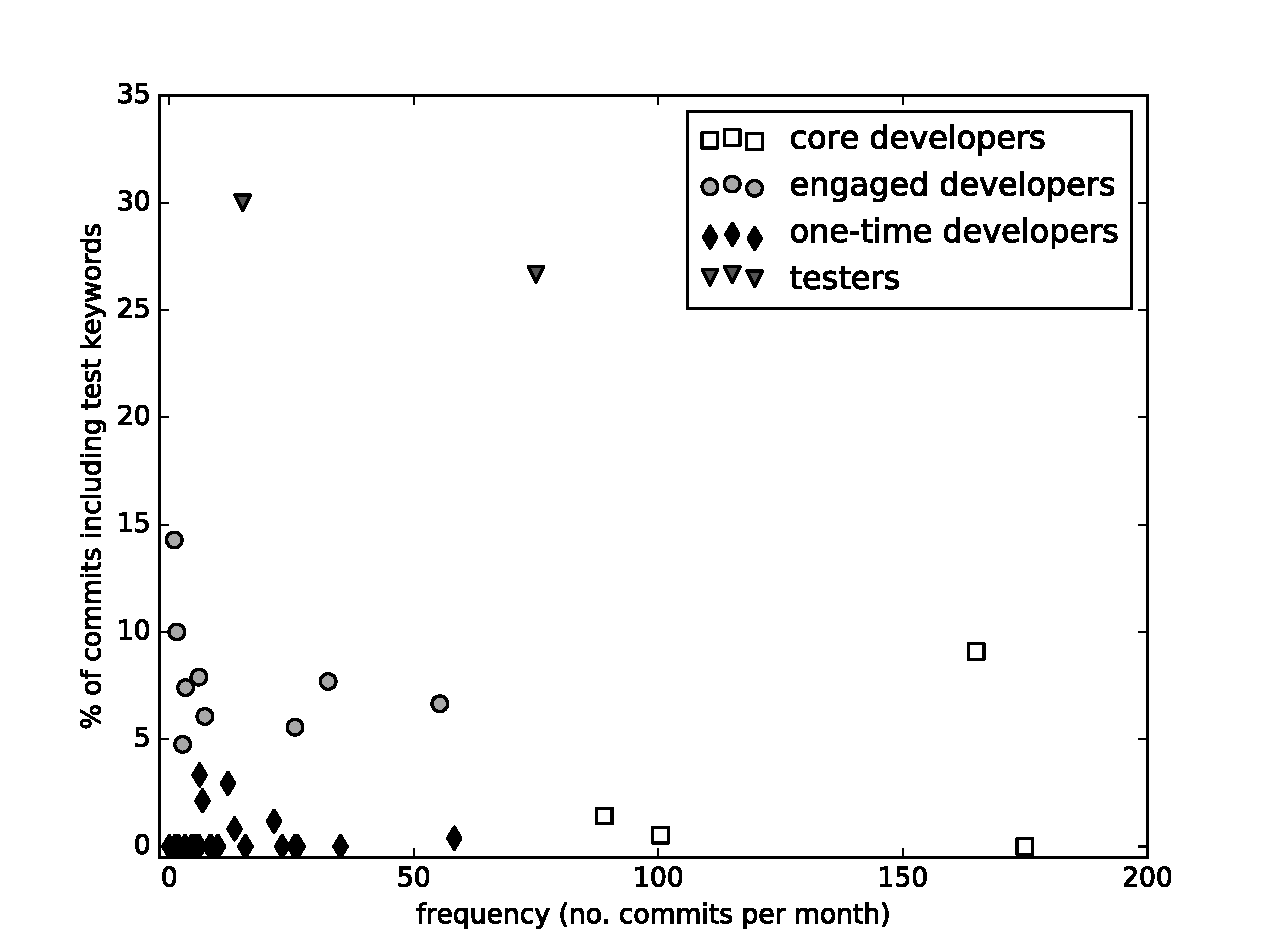
\includegraphics[width=\columnwidth]{ResourceClassification/figures/prom4k_black.pdf}
   \caption{Scatterplot with color-coded clusters, ProM data set}
   \label{fig:prom4k}
\end{figure}

%\todo{shorten to fit into 1 column}

The Camunda data set was analyzed based on the optimal features and classes derived of the Infinica data set. The majority of the users are developers like in the ProM data set. However, it is an open source project and users can commit anything at any time without restrictions. There is a permanently appointed core team which evaluates, selects and integrates commits for the product. The clustering creates similar classes like in the ProM data set and it can be divided into the following four classes as shown in \Cref{fig:camunda4k}.

\begin{itemize}

\item \textbf{Core developers:} The square cluster contains the employed users of the Camunda project. Their commit frequency and absolute number commits is far above the others.

\item \textbf{Engaged developers:} Developers which stay longer with the project are situated in the circle cluster. They are refining their own committed code or they are extending the product in different areas.

\item \textbf{One-time developers:} Similar to the ProM data set the majority of the users belongs to this group and it is represented by the diamond cluster. Code usefull or not is committed typically once and there is no lasting commitment.

\item \textbf{Testers:} Also testers have been identified in the triangle cluster. They already have a lower frequency than developers and therefore it is difficult to make an estimation about their commitment.

\end{itemize}

\begin{figure}
   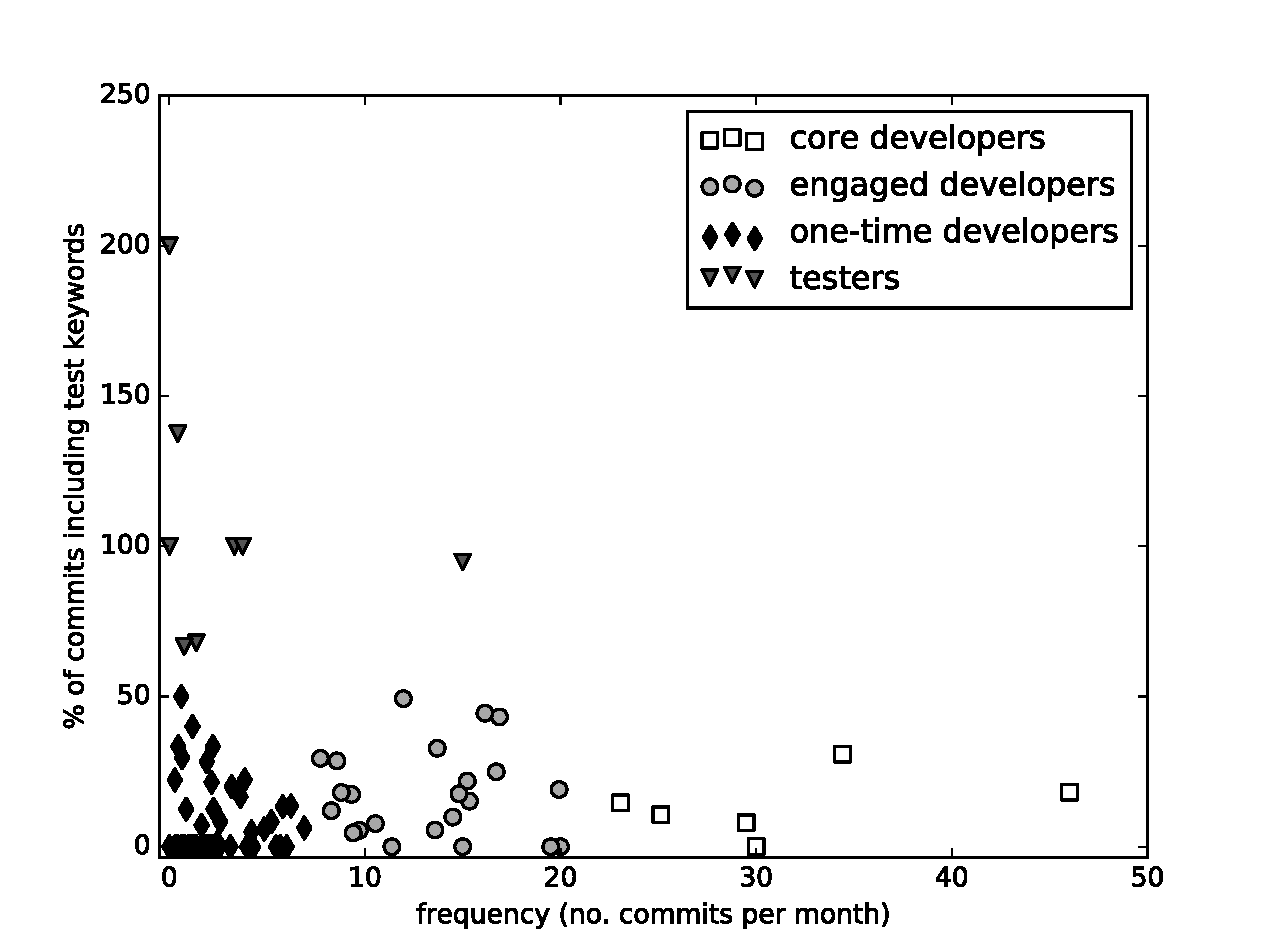
\includegraphics[width=\columnwidth]{ResourceClassification/figures/camunda4k_black.pdf}
   \caption{Scatterplot with colorcoded clusters, Camunda data set}
   \label{fig:camunda4k}
\end{figure}

For the user-based approach no further distinction can be made based on expertise, time in the company, teamwork, development area, project membership, room allocation, etc. In the case of a development from junior to a senior role in the course of the coverage of the log file the respective persons stay within their previous clusters. The associated increase or decrease in commit frequency can not be linked to the development. %since the observations developed in opposite directions.


\begin{figure}
   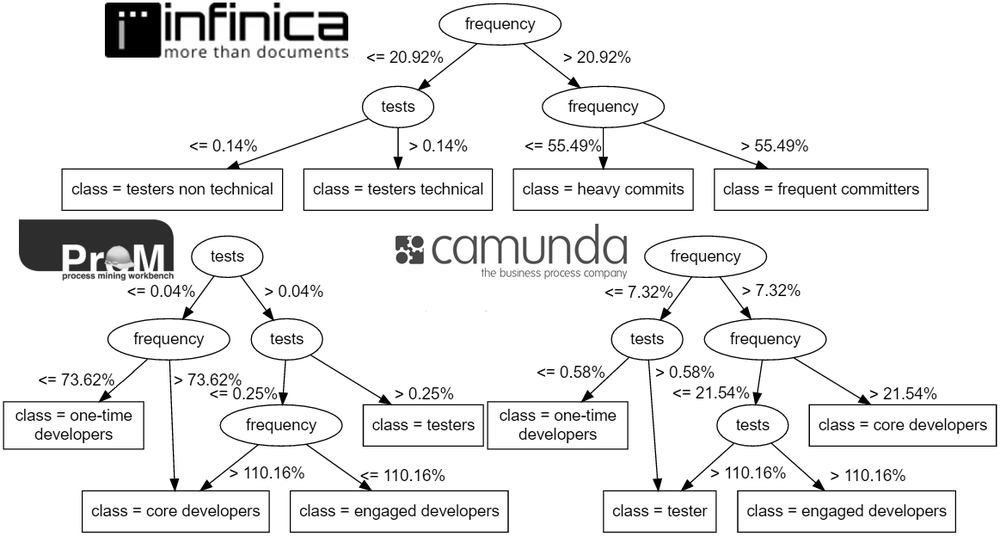
\includegraphics[width=\columnwidth]{ResourceClassification/figures/4ktrees.png}
   \caption{Decision trees, all three data sets}\
   \label{fig:trees}
\end{figure}


Decision trees are an effective tool to display the formation and partitioning of clusters in a tree-like model. The corresponding decision trees for the previous presented k-means clustering shown in \Cref{fig:trees} display the boundaries of the clusters. Due to the differences in the structure of the projects, business vs open source, the data sets share only little similarities.

The Infinica decision tree initially splits the developers and the testers apart based on the commit frequency with a border value of 20.92\%. The developers are split again into subclasses based on the commit frequency, which now separates them at 55.49\% into frequent committers and heavy commits. The testers are split based on test related word occurrences at 0.14\%, where the non technical testers use these words less often than their technical counterparts. On the contrary, the other two trees start separating the subsets right away in different orders without displaying a clean separation between developers and testers from the beginning.

The decision tree model for the commit-based approach is depicted in \Cref{fig:tree}. When comparing its rules with those of our manual classification there are some clear parallels. In the tree the differentiation between web developers and other developers is done with a border value of 36\% for web commits, close to the 40\% threshold of the manual table. Testers are identified having more than 17\% test commits, similar to the 20\% boundary. The decision tree separates the support users from the rest using the vcsManagement type. Looking at the data, this rule is definitely valid for the Infinica data, however as we were not able to provide a definite explanation for this class having higher percentages for that particular type, we can not say if this rule would also apply to other data sets. One possible explanation is that all users have a similar number of vcsManagement commits within a given timeframe, but because the support role has on average a significantly lower number of commits, they account for a higher percentage in the distribution, however this is only an assumption.

\begin{figure}
	\centering
	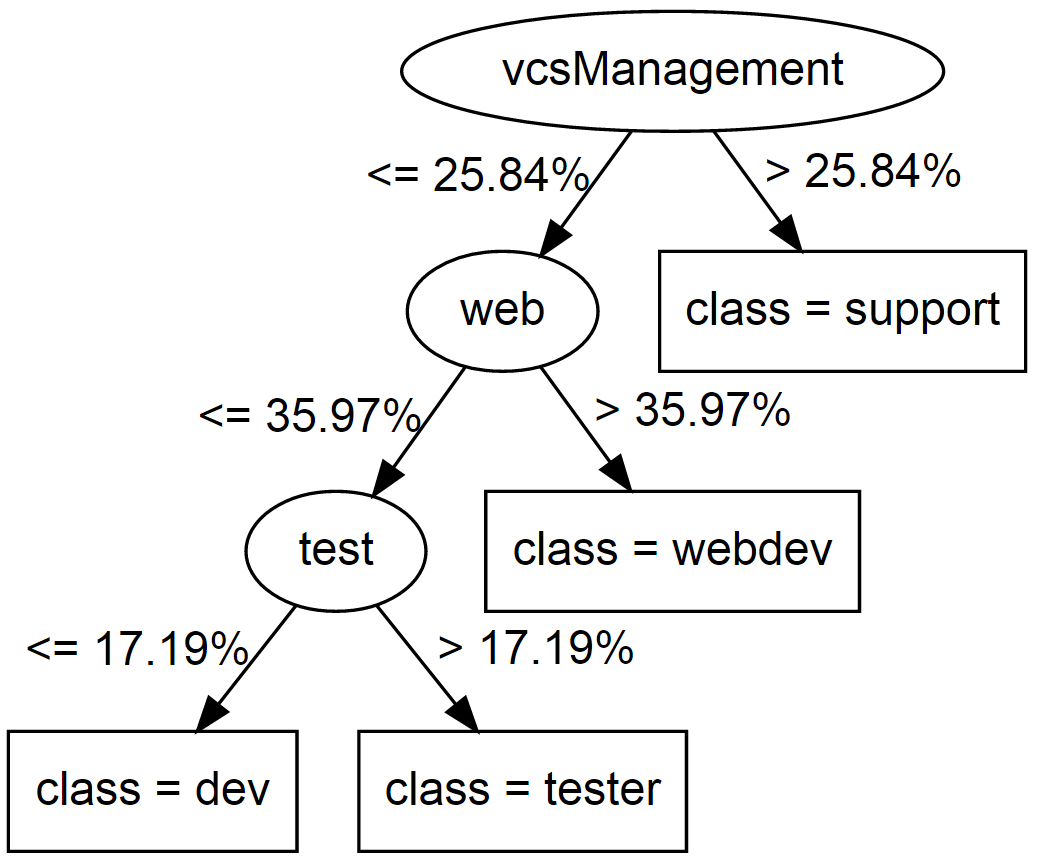
\includegraphics[width=0.6\columnwidth]{ResourceClassification/figures/commit_tree.png}
	\caption{Decision tree, commit based model}
	\label{fig:tree}
\end{figure}

In general the decision tree is more precise, but our manually created rules capture more factors of differentiation and we were able to identify some potential classes which could not be included in the programmatic classification with reasonable effort. A clear advantage of the automated model is that it can be efficiently applied to other data sets. Applying it to the Camunda and ProM data sets provided some verification for our decision tree model. We only included users with five or more commits into the cross validation. For the Prom data set which consisted of 42 users, 35 (83\%) were classified
as developers. This is not surprising as we knew before that the contributors
of open source projects are mostly developers, which was also confirmed by our
contact persons for ProM and Camunda. Six (14\%) were regarded as testers,
which fits to our results in the user-based approach. One remaining user (2\%) was classified as a web developer. As the ProM project has no web component, it makes sense that there are no web developers found by our algorithm. The one we found has only five commits, two of them web commits so this potential misclassification provides no evidence against the quality of the overall approach.

\begin{figure*}[h!t]
	\begin{subfigure}[t]{.5\linewidth}
		\centering
		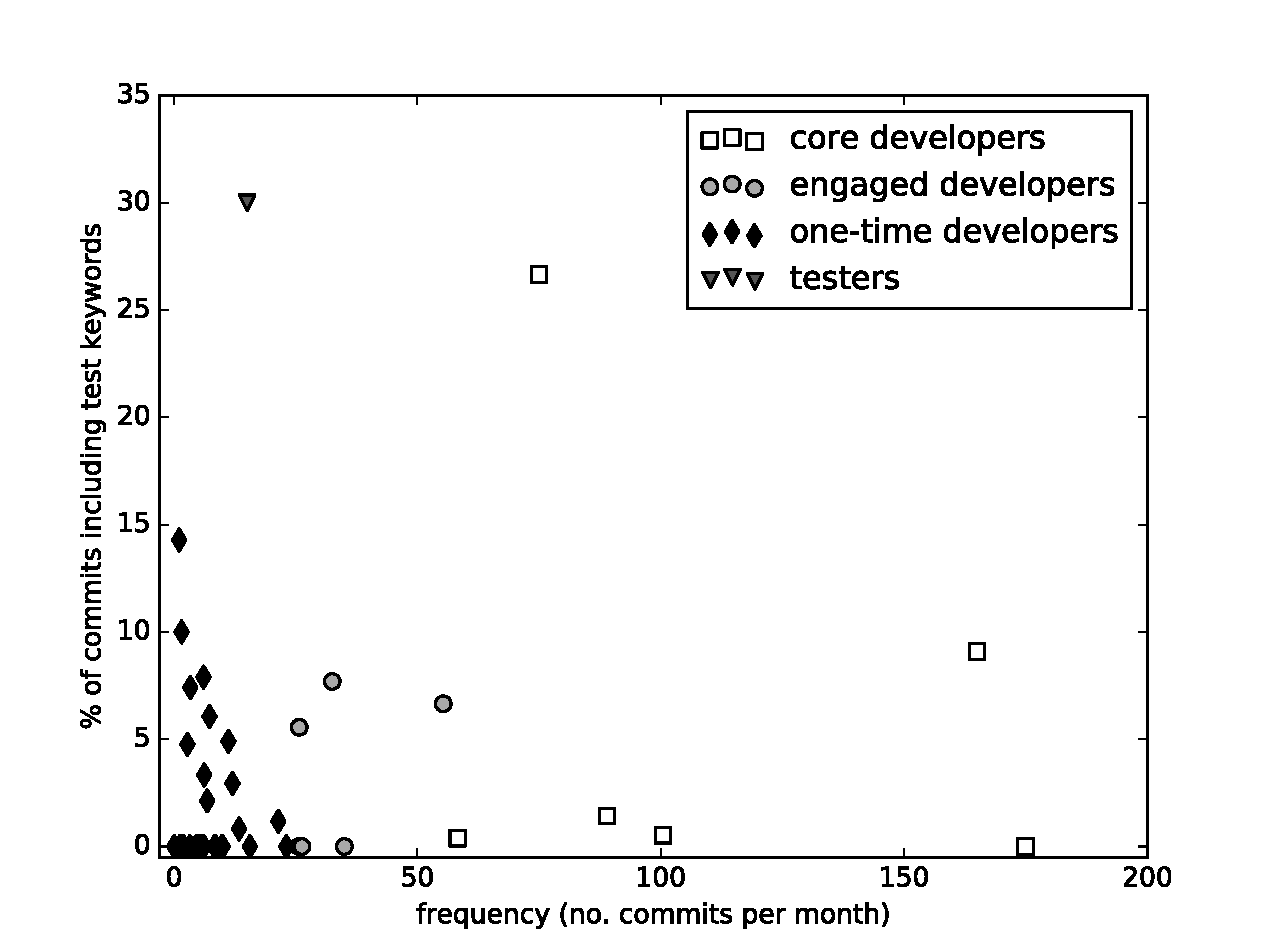
\includegraphics[width=\textwidth]{ResourceClassification/figures/infinica4kpredict_prom_black.pdf}
	\end{subfigure}
	\begin{subfigure}[t]{.5\linewidth}
		\centering
		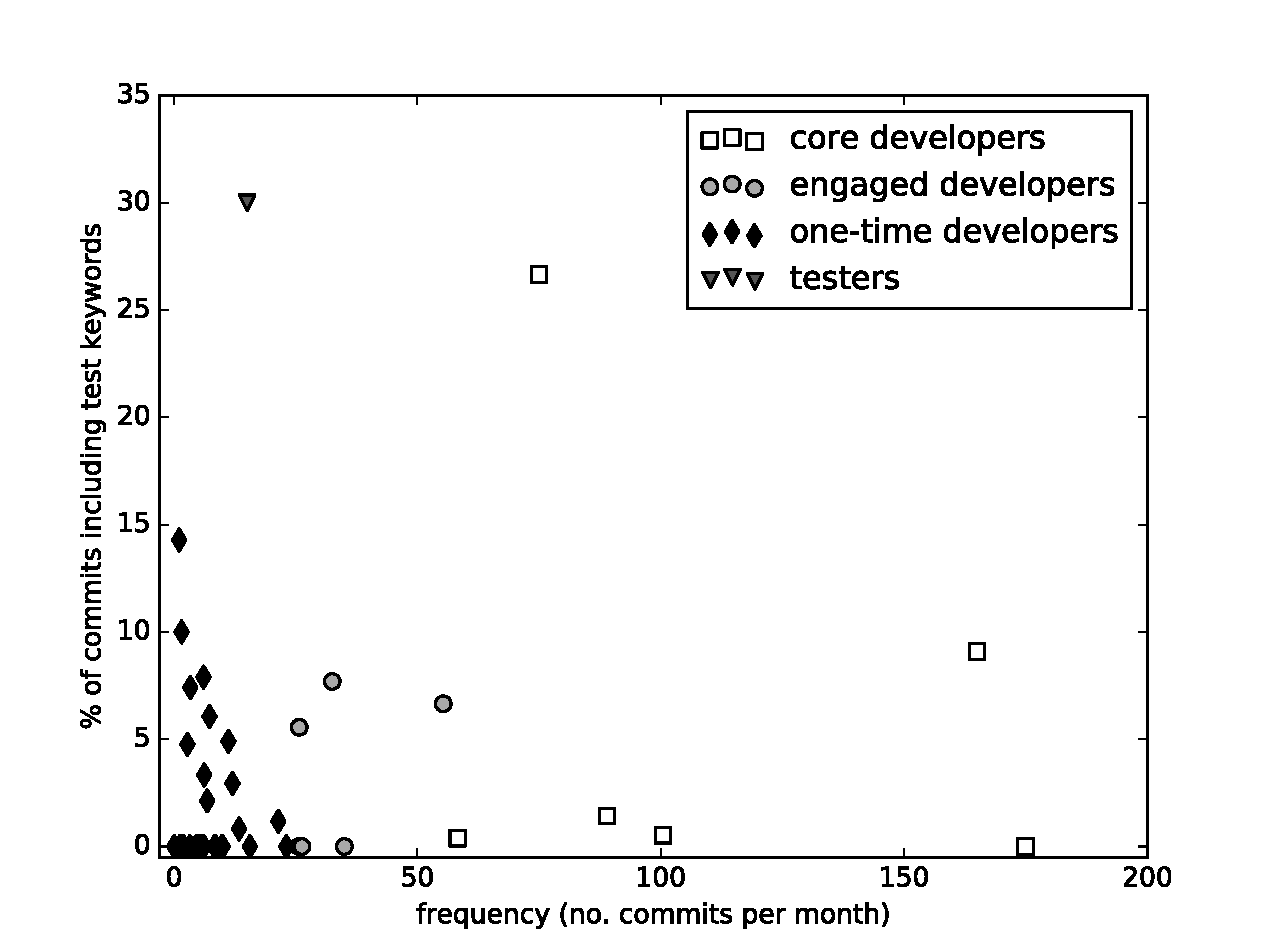
\includegraphics[width=\textwidth]{ResourceClassification/figures/infinica4kpredict_prom_black.pdf}
	\end{subfigure}
	\caption{Classication based on Infinica training set: Prom, Camunda}
	\label{fig:infinica-predict}
\end{figure*}

For the Camunda data the case is similar. Out of 66 total users, 49 (74\%)
percent were regarded as developers, the high number is again explained by the
type of project and was confirmed by the contact person we interviewed. 10 (15\%)
testers were found, also mostly fitting to our knowledge of the data. Contrary
to ProM, there is a web part in the analyzed Camunda project reflected by the
fact that our algorithm found 7 (11\%) web developers. In neither of the two validation data sets a support user was found. This might be due to the differences in the organisational structure between Infinica and the other two or it could stem from the classification rule based on the vcsManagement commit type, which we already discussed as potential source of error. All users in the Camunda and ProM data have below 15 percent vcsManagement commits, too small to fit the support class generated by the decision tree model. However there are other commit types with high percentages, such as build or toolManagement, in Camunda and Prom, which might fit the support class or a similar one.

When validating the model with the Infinica data set and then predicting the ProM and Campunda data set, only moderate results are achieved with the user-based approach as shown in \Cref{fig:infinica-predict}. For the Infinica data set meaningful classes can not be conveyed to the other data sets due to the structural differences of the projects.


For ProM (\Cref{fig:infinica-predict} left) the trained classes are less representative than the ones created when clustering on its own, especially since the ProM data set does not include any designated testers. The prediction of Camunda (\Cref{fig:infinica-predict} right) on the other hand performs better. However, the core developer class now also includes very committed contributors.

Because of the missing designated testers in both test data sets, the initial differentiation between technical and non-technical testers is not possible. Due to the moderate results of user based approach the commit based approach was initiated.



%\section{Future Work}
%the preliminary stage on which we plan to build upon a more comprehensive solution of the problem of role discovery from \gls*{vcs}. 
%There are many ways to extend our approaches as well as other potential methodologies for classification. 
%On the technical level, different methods of clustering and classification from the machine learning domain could be used. More conceptual additions would be for example the use of additional features and feature combinations.

%In this research we focused mainly on the user roles for classification but there might be other classes, for example differentiated by experience of users. 
%We expect improvement potential by analyzing different categories of VCS repositories. Especially log files of large software companies, where many different roles are formally defined and executed would be interesting.

%There is also much potential for further refining our proposed methods. For instance, we would use more extensively the natural language toolkit for processing the commit messages. So far we only used the more basic functionality of the language processing tools. In this research we focused mainly on the user roles for classification but there might be other classes, for example discriminated by the experience of users. Significant improvements would be possible by analyzing different categories of VCS repositories. Especially log files of large software companies, where many different roles are formally defined and executed would be interesting.

\section{Conclusion and Future Work}\label{sec:conclusion}
We presented a first approach to resource classification from \gls*{vcs} and demonstrated feasibility of this non-trivial task. The data saved in log files contains much useful information. But in particular the structure of the underlying team and project has a big influence on finding classes and their identified attributes. Further, the many differences between individual repositories make it difficult to generalize findings.

Automating the classification with machine learning is a viable method. Even though not all required steps of creating the classification models can be done automatically and further information about the users and structure is essential. Despite current challenges, the users can be classified to a certain extent. A more precise classification, however, requires future research. One direction is to further explore clustering and classification techniques to find better suited techniques. Finally, an extension of the approach with state-of-the-art semantic reasoning seems a promising vein of research to the authors.

\section*{Acknowledgment}
This work has been funded by the Austrian Research Promotion Agency (FFG)
under grant 845638 (SHAPE) and the European Union’s Seventh Framework Programme under grant 612052 (SERAMIS).

\bibliographystyle{IEEEtran}
\bibliography{Bibliography}

\end{document}